\newcommand{\drawpintegration}{\[\int udv=uv-\int vdu\]}
\newcommand{\fconstu}{z^3}
\newcommand{\fconstdu}{3z^2dz}
\newcommand{\fconstdv}{e^zdz}
\newcommand{\fconstv}{e^z}
\newcommand{\fintsolution}{\int z^2e^zdz}
\newcommand{\fsolution}{\int z^2e^zdz}
\newcommand{\sconstu}{z^2}
\newcommand{\sconstdu}{2zdz}
\newcommand{\sconstdv}{e^zdz}
\newcommand{\sconstv}{e^z}
\newcommand{\sintsolution}{\int ze^zdz}
\newcommand{\ssolution}{e^z(z^2-2z+2)}
\newcommand{\tconstu}{z}
\newcommand{\tconstdu}{dz}
\newcommand{\tconstdv}{e^zdz}
\newcommand{\tconstv}{e^z}
\newcommand{\tsolution}{e^z(z-1)}

\textbf{Temática 2 - Método integración por partes}
\[\int z^3e^zdz\]
\[
    \begin{matrix}
        u=\fconstu & du=\fconstdu \\
        dv=\fconstdv & v=\fconstv
    \end{matrix}
\]

\drawpintegration
\[\int \fconstu \fconstdv=\fconstu \fconstv-\int \fconstv \fconstdu\]
\[\int \fconstu \fconstdv=\fconstu \fconstv-3\fintsolution\]
\[
    \begin{aligned}
        Derivamos && \fintsolution
    \end{aligned}
\]

\[
    \begin{matrix}
        u=\sconstu & du=\sconstdu \\
        dv=\sconstdv & v=\sconstv
    \end{matrix}
\]

\drawpintegration
\[\int \sconstu \sconstdv=\sconstu \sconstv-\int \sconstv \sconstdu\]
\[\int \sconstu \sconstdv=\sconstu \sconstv-2\sintsolution\]
\[
    \begin{aligned}
        Derivamos && \sintsolution
    \end{aligned}
\]

\[
    \begin{matrix}
        u=\tconstu & du=\tconstdu \\
        dv=\tconstdv & v=\tconstv
    \end{matrix}
\]

\drawpintegration
\[\int \tconstu \tconstdv=\tconstu \tconstv-\int \tconstv \tconstdu\]
\[\int \tconstu \tconstdv=\tconstu \tconstv-e^z\]
\[\int \tconstu \tconstdv=\tsolution\]
\[
    \begin{aligned}
        Remplazamos && \tsolution && en && \sintsolution
    \end{aligned}
\]

\[\int \sconstu \sconstdv=\sconstu \sconstv-2(\tsolution)\]
\[\int \sconstu \sconstdv=\sconstu \sconstv-2\tsolution\]
\[\int \sconstu \sconstdv=\sconstu \sconstv-2ze^z+2e\]
\[\int \sconstu \sconstdv=\ssolution\]
\[
    \begin{aligned}
        Remplazamos && \ssolution && en && \fintsolution
    \end{aligned}
\]

\[\int \fconstu \fconstdv=\fconstu \fconstv-3\ssolution\]
\[\int \fconstu \fconstdv=\fconstu \fconstv-3z^2e^z+6ze^z-6e^z\]
\[\int \fconstu \fconstdv=e^z(z^3-3z^2+6z-6)+C\]

\begin{figure}[h]
    \begin{center}
        \fbox{
            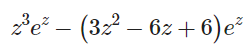
\includegraphics{comp-task2.png}
        }
        \caption{Integración por partes sympy}
    \end{center}
\end{figure}